\documentclass[12pt]{extarticle}
\usepackage[letterpaper,top=20mm,bottom=20mm,left=16mm,right=16mm,headheight=16pt,headsep=7mm,footskip=10mm]{geometry}
\usepackage[T1]{fontenc}
\usepackage{tgheros}
\renewcommand{\familydefault}{\sfdefault}
\usepackage{tikz}
\usetikzlibrary{arrows.meta,decorations.pathreplacing}
\usepackage{fancyhdr}
\usepackage{xcolor}
\definecolor{cardred}{RGB}{206,38,38}
\definecolor{cardblue}{RGB}{28,92,196}
\colorlet{stripred}{cardred!32}
\colorlet{stripblue}{cardblue!28}
\colorlet{panelgrey}{black!20}
\colorlet{boxgrey}{black!45}
\tikzset{cardedge/.style={draw=black!70,line width=0.5pt}}
\pagestyle{fancy}
\fancyhf{}
\fancyhead[L]{\small Week 58 / Fair division / Grades 4--5}
\fancyfoot[L]{\small Bellingham Math Circle / Week 58 / W58-RV-U-v1}
\fancyfoot[R]{\small \thepage}
\renewcommand{\headrulewidth}{0.4pt}
\renewcommand{\footrulewidth}{0pt}
\setlength{\parindent}{0pt}
\setlength{\parskip}{4pt}
\newcommand{\prob}[1]{\par\noindent\textbf{Problem #1:} }
\begin{document}
A train is a row of goods cards. To share a train, cut it at some of the gaps between neighbouring cards, so that every card stays whole, and put each piece into one of two trays. A tray may get more than one piece. Both trays must get the same number of red cards and the same number of blue cards.
\begin{center}
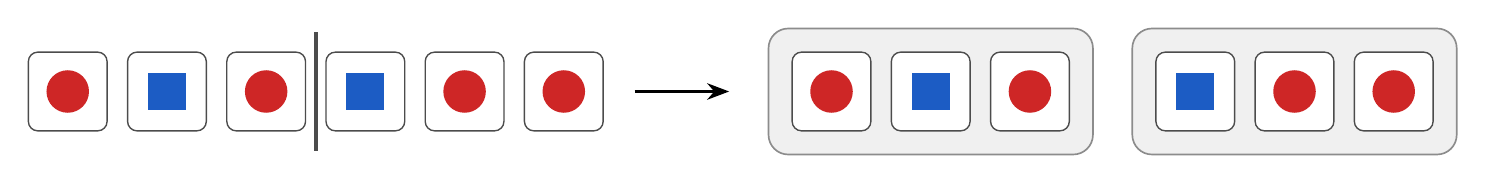
\begin{tikzpicture}[x=1mm,y=1mm]
\draw[cardedge, fill=white, rounded corners=1.2mm] (0,0) rectangle (10,10);
\fill[cardred] (5,5) circle (2.7mm);
\draw[cardedge, fill=white, rounded corners=1.2mm] (12.6,0) rectangle (22.6,10);
\fill[cardblue] (15.2,2.6) rectangle (20,7.4);
\draw[cardedge, fill=white, rounded corners=1.2mm] (25.2,0) rectangle (35.2,10);
\fill[cardred] (30.2,5) circle (2.7mm);
\draw[cardedge, fill=white, rounded corners=1.2mm] (37.8,0) rectangle (47.8,10);
\fill[cardblue] (40.4,2.6) rectangle (45.2,7.4);
\draw[cardedge, fill=white, rounded corners=1.2mm] (50.4,0) rectangle (60.4,10);
\fill[cardred] (55.4,5) circle (2.7mm);
\draw[cardedge, fill=white, rounded corners=1.2mm] (63,0) rectangle (73,10);
\fill[cardred] (68,5) circle (2.7mm);
\draw[black!70, line width=1.4pt] (36.5,-2.5) -- (36.5,12.5);
\draw[-{Stealth[length=2.8mm]}, line width=0.9pt] (77,5) -- (89,5);
\draw[black!45, fill=black!6, line width=0.6pt, rounded corners=2.5mm] (94,-3) rectangle (135.2,13);
\draw[cardedge, fill=white, rounded corners=1.2mm] (97,0) rectangle (107,10);
\fill[cardred] (102,5) circle (2.7mm);
\draw[cardedge, fill=white, rounded corners=1.2mm] (109.6,0) rectangle (119.6,10);
\fill[cardblue] (112.2,2.6) rectangle (117,7.4);
\draw[cardedge, fill=white, rounded corners=1.2mm] (122.2,0) rectangle (132.2,10);
\fill[cardred] (127.2,5) circle (2.7mm);
\draw[black!45, fill=black!6, line width=0.6pt, rounded corners=2.5mm] (140.2,-3) rectangle (181.4,13);
\draw[cardedge, fill=white, rounded corners=1.2mm] (143.2,0) rectangle (153.2,10);
\fill[cardblue] (145.8,2.6) rectangle (150.6,7.4);
\draw[cardedge, fill=white, rounded corners=1.2mm] (155.8,0) rectangle (165.8,10);
\fill[cardred] (160.8,5) circle (2.7mm);
\draw[cardedge, fill=white, rounded corners=1.2mm] (168.4,0) rectangle (178.4,10);
\fill[cardred] (173.4,5) circle (2.7mm);
\end{tikzpicture}
\end{center}
\vspace{1mm}
\prob{1}Share each of these trains with as few cuts as you can. How can you tell, without trying, whether a train of four red cards and four blue cards can be shared with one cut?
\vspace{3mm}
\begin{center}
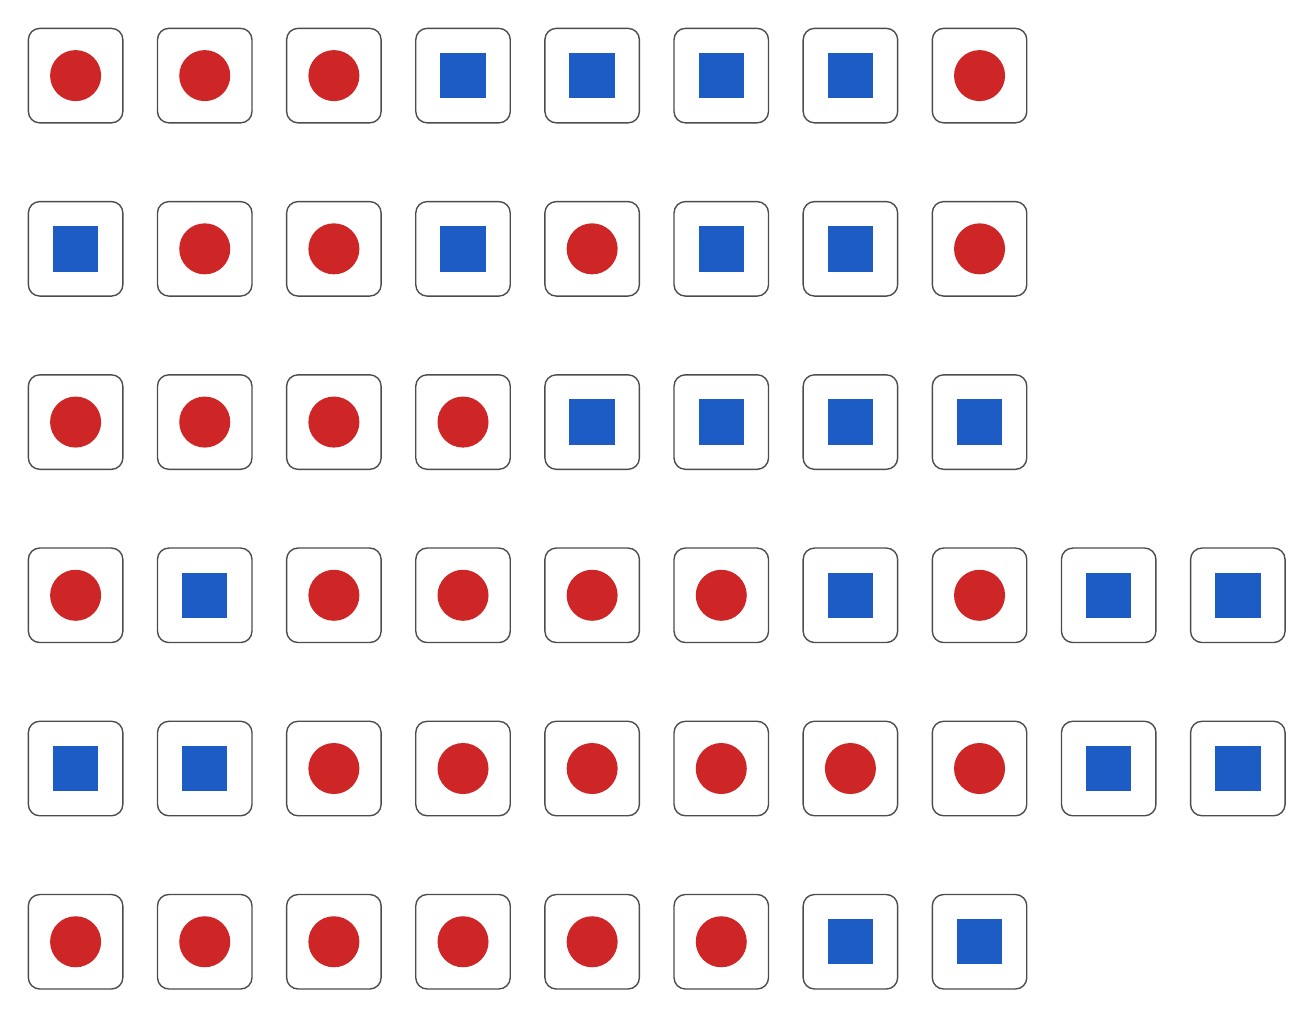
\begin{tikzpicture}[x=1mm,y=1mm]
\draw[cardedge, fill=white, rounded corners=1.44mm] (0,0) rectangle (12,12);
\fill[cardred] (6,6) circle (3.24mm);
\draw[cardedge, fill=white, rounded corners=1.44mm] (16.4,0) rectangle (28.4,12);
\fill[cardred] (22.4,6) circle (3.24mm);
\draw[cardedge, fill=white, rounded corners=1.44mm] (32.8,0) rectangle (44.8,12);
\fill[cardred] (38.8,6) circle (3.24mm);
\draw[cardedge, fill=white, rounded corners=1.44mm] (49.2,0) rectangle (61.2,12);
\fill[cardblue] (52.32,3.12) rectangle (58.08,8.88);
\draw[cardedge, fill=white, rounded corners=1.44mm] (65.6,0) rectangle (77.6,12);
\fill[cardblue] (68.72,3.12) rectangle (74.48,8.88);
\draw[cardedge, fill=white, rounded corners=1.44mm] (82,0) rectangle (94,12);
\fill[cardblue] (85.12,3.12) rectangle (90.88,8.88);
\draw[cardedge, fill=white, rounded corners=1.44mm] (98.4,0) rectangle (110.4,12);
\fill[cardblue] (101.52,3.12) rectangle (107.28,8.88);
\draw[cardedge, fill=white, rounded corners=1.44mm] (114.8,0) rectangle (126.8,12);
\fill[cardred] (120.8,6) circle (3.24mm);
\draw[cardedge, fill=white, rounded corners=1.44mm] (0,-22) rectangle (12,-10);
\fill[cardblue] (3.12,-18.88) rectangle (8.88,-13.12);
\draw[cardedge, fill=white, rounded corners=1.44mm] (16.4,-22) rectangle (28.4,-10);
\fill[cardred] (22.4,-16) circle (3.24mm);
\draw[cardedge, fill=white, rounded corners=1.44mm] (32.8,-22) rectangle (44.8,-10);
\fill[cardred] (38.8,-16) circle (3.24mm);
\draw[cardedge, fill=white, rounded corners=1.44mm] (49.2,-22) rectangle (61.2,-10);
\fill[cardblue] (52.32,-18.88) rectangle (58.08,-13.12);
\draw[cardedge, fill=white, rounded corners=1.44mm] (65.6,-22) rectangle (77.6,-10);
\fill[cardred] (71.6,-16) circle (3.24mm);
\draw[cardedge, fill=white, rounded corners=1.44mm] (82,-22) rectangle (94,-10);
\fill[cardblue] (85.12,-18.88) rectangle (90.88,-13.12);
\draw[cardedge, fill=white, rounded corners=1.44mm] (98.4,-22) rectangle (110.4,-10);
\fill[cardblue] (101.52,-18.88) rectangle (107.28,-13.12);
\draw[cardedge, fill=white, rounded corners=1.44mm] (114.8,-22) rectangle (126.8,-10);
\fill[cardred] (120.8,-16) circle (3.24mm);
\draw[cardedge, fill=white, rounded corners=1.44mm] (0,-44) rectangle (12,-32);
\fill[cardred] (6,-38) circle (3.24mm);
\draw[cardedge, fill=white, rounded corners=1.44mm] (16.4,-44) rectangle (28.4,-32);
\fill[cardred] (22.4,-38) circle (3.24mm);
\draw[cardedge, fill=white, rounded corners=1.44mm] (32.8,-44) rectangle (44.8,-32);
\fill[cardred] (38.8,-38) circle (3.24mm);
\draw[cardedge, fill=white, rounded corners=1.44mm] (49.2,-44) rectangle (61.2,-32);
\fill[cardred] (55.2,-38) circle (3.24mm);
\draw[cardedge, fill=white, rounded corners=1.44mm] (65.6,-44) rectangle (77.6,-32);
\fill[cardblue] (68.72,-40.88) rectangle (74.48,-35.12);
\draw[cardedge, fill=white, rounded corners=1.44mm] (82,-44) rectangle (94,-32);
\fill[cardblue] (85.12,-40.88) rectangle (90.88,-35.12);
\draw[cardedge, fill=white, rounded corners=1.44mm] (98.4,-44) rectangle (110.4,-32);
\fill[cardblue] (101.52,-40.88) rectangle (107.28,-35.12);
\draw[cardedge, fill=white, rounded corners=1.44mm] (114.8,-44) rectangle (126.8,-32);
\fill[cardblue] (117.92,-40.88) rectangle (123.68,-35.12);
\draw[cardedge, fill=white, rounded corners=1.44mm] (0,-66) rectangle (12,-54);
\fill[cardred] (6,-60) circle (3.24mm);
\draw[cardedge, fill=white, rounded corners=1.44mm] (16.4,-66) rectangle (28.4,-54);
\fill[cardblue] (19.52,-62.88) rectangle (25.28,-57.12);
\draw[cardedge, fill=white, rounded corners=1.44mm] (32.8,-66) rectangle (44.8,-54);
\fill[cardred] (38.8,-60) circle (3.24mm);
\draw[cardedge, fill=white, rounded corners=1.44mm] (49.2,-66) rectangle (61.2,-54);
\fill[cardred] (55.2,-60) circle (3.24mm);
\draw[cardedge, fill=white, rounded corners=1.44mm] (65.6,-66) rectangle (77.6,-54);
\fill[cardred] (71.6,-60) circle (3.24mm);
\draw[cardedge, fill=white, rounded corners=1.44mm] (82,-66) rectangle (94,-54);
\fill[cardred] (88,-60) circle (3.24mm);
\draw[cardedge, fill=white, rounded corners=1.44mm] (98.4,-66) rectangle (110.4,-54);
\fill[cardblue] (101.52,-62.88) rectangle (107.28,-57.12);
\draw[cardedge, fill=white, rounded corners=1.44mm] (114.8,-66) rectangle (126.8,-54);
\fill[cardred] (120.8,-60) circle (3.24mm);
\draw[cardedge, fill=white, rounded corners=1.44mm] (131.2,-66) rectangle (143.2,-54);
\fill[cardblue] (134.32,-62.88) rectangle (140.08,-57.12);
\draw[cardedge, fill=white, rounded corners=1.44mm] (147.6,-66) rectangle (159.6,-54);
\fill[cardblue] (150.72,-62.88) rectangle (156.48,-57.12);
\draw[cardedge, fill=white, rounded corners=1.44mm] (0,-88) rectangle (12,-76);
\fill[cardblue] (3.12,-84.88) rectangle (8.88,-79.12);
\draw[cardedge, fill=white, rounded corners=1.44mm] (16.4,-88) rectangle (28.4,-76);
\fill[cardblue] (19.52,-84.88) rectangle (25.28,-79.12);
\draw[cardedge, fill=white, rounded corners=1.44mm] (32.8,-88) rectangle (44.8,-76);
\fill[cardred] (38.8,-82) circle (3.24mm);
\draw[cardedge, fill=white, rounded corners=1.44mm] (49.2,-88) rectangle (61.2,-76);
\fill[cardred] (55.2,-82) circle (3.24mm);
\draw[cardedge, fill=white, rounded corners=1.44mm] (65.6,-88) rectangle (77.6,-76);
\fill[cardred] (71.6,-82) circle (3.24mm);
\draw[cardedge, fill=white, rounded corners=1.44mm] (82,-88) rectangle (94,-76);
\fill[cardred] (88,-82) circle (3.24mm);
\draw[cardedge, fill=white, rounded corners=1.44mm] (98.4,-88) rectangle (110.4,-76);
\fill[cardred] (104.4,-82) circle (3.24mm);
\draw[cardedge, fill=white, rounded corners=1.44mm] (114.8,-88) rectangle (126.8,-76);
\fill[cardred] (120.8,-82) circle (3.24mm);
\draw[cardedge, fill=white, rounded corners=1.44mm] (131.2,-88) rectangle (143.2,-76);
\fill[cardblue] (134.32,-84.88) rectangle (140.08,-79.12);
\draw[cardedge, fill=white, rounded corners=1.44mm] (147.6,-88) rectangle (159.6,-76);
\fill[cardblue] (150.72,-84.88) rectangle (156.48,-79.12);
\draw[cardedge, fill=white, rounded corners=1.44mm] (0,-110) rectangle (12,-98);
\fill[cardred] (6,-104) circle (3.24mm);
\draw[cardedge, fill=white, rounded corners=1.44mm] (16.4,-110) rectangle (28.4,-98);
\fill[cardred] (22.4,-104) circle (3.24mm);
\draw[cardedge, fill=white, rounded corners=1.44mm] (32.8,-110) rectangle (44.8,-98);
\fill[cardred] (38.8,-104) circle (3.24mm);
\draw[cardedge, fill=white, rounded corners=1.44mm] (49.2,-110) rectangle (61.2,-98);
\fill[cardred] (55.2,-104) circle (3.24mm);
\draw[cardedge, fill=white, rounded corners=1.44mm] (65.6,-110) rectangle (77.6,-98);
\fill[cardred] (71.6,-104) circle (3.24mm);
\draw[cardedge, fill=white, rounded corners=1.44mm] (82,-110) rectangle (94,-98);
\fill[cardred] (88,-104) circle (3.24mm);
\draw[cardedge, fill=white, rounded corners=1.44mm] (98.4,-110) rectangle (110.4,-98);
\fill[cardblue] (101.52,-106.88) rectangle (107.28,-101.12);
\draw[cardedge, fill=white, rounded corners=1.44mm] (114.8,-110) rectangle (126.8,-98);
\fill[cardblue] (117.92,-106.88) rectangle (123.68,-101.12);
\path (0,0) -- (159.6,0);
\end{tikzpicture}
\end{center}
\newpage
\prob{2}Can a train with an even number of red cards and an even number of blue cards ever need more than two cuts? Explain.
\vspace{88mm}
\prob{3}One person uses the two-person card A, and another person uses the two-person card B.
\begin{center}
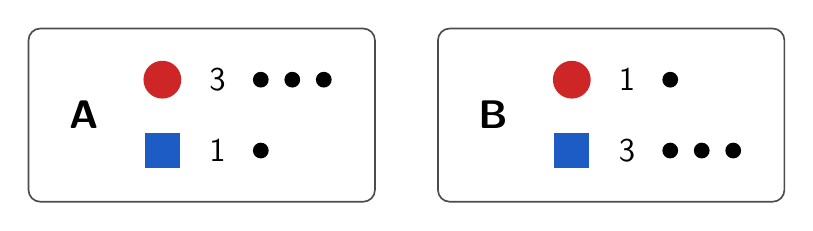
\begin{tikzpicture}[x=1mm,y=1mm]
\draw[black!70, line width=0.6pt, rounded corners=1.5mm] (0,0) rectangle (44,22);
\node[font=\Large\bfseries] at (7,11) {A};
\fill[cardred] (17,15.5) circle (2.4mm);
\node[font=\large] at (24,15.5) {3};
\fill[black] (29.5,15.5) circle (1mm);
\fill[black] (33.5,15.5) circle (1mm);
\fill[black] (37.5,15.5) circle (1mm);
\fill[cardblue] (14.8,4.3) rectangle (19.2,8.7);
\node[font=\large] at (24,6.5) {1};
\fill[black] (29.5,6.5) circle (1mm);
\draw[black!70, line width=0.6pt, rounded corners=1.5mm] (52,0) rectangle (96,22);
\node[font=\Large\bfseries] at (59,11) {B};
\fill[cardred] (69,15.5) circle (2.4mm);
\node[font=\large] at (76,15.5) {1};
\fill[black] (81.5,15.5) circle (1mm);
\fill[cardblue] (66.8,4.3) rectangle (71.2,8.7);
\node[font=\large] at (76,6.5) {3};
\fill[black] (81.5,6.5) circle (1mm);
\fill[black] (85.5,6.5) circle (1mm);
\fill[black] (89.5,6.5) circle (1mm);
\end{tikzpicture}
\end{center}
On a strip, each number is the value of the whole 120\,mm panel of that colour, and value follows length: 40\,mm of red is worth 1 to A. Every cut goes straight across the strip. Share one strip between two trays so that A finds the two trays worth the same, and B does too. Use as few cuts as you can, and explain why fewer cuts cannot work. Is there more than one way to do it with that many cuts? If the two people held cards with any other numbers, could two cuts always do it? Explain.
\vspace{5mm}
\begin{center}
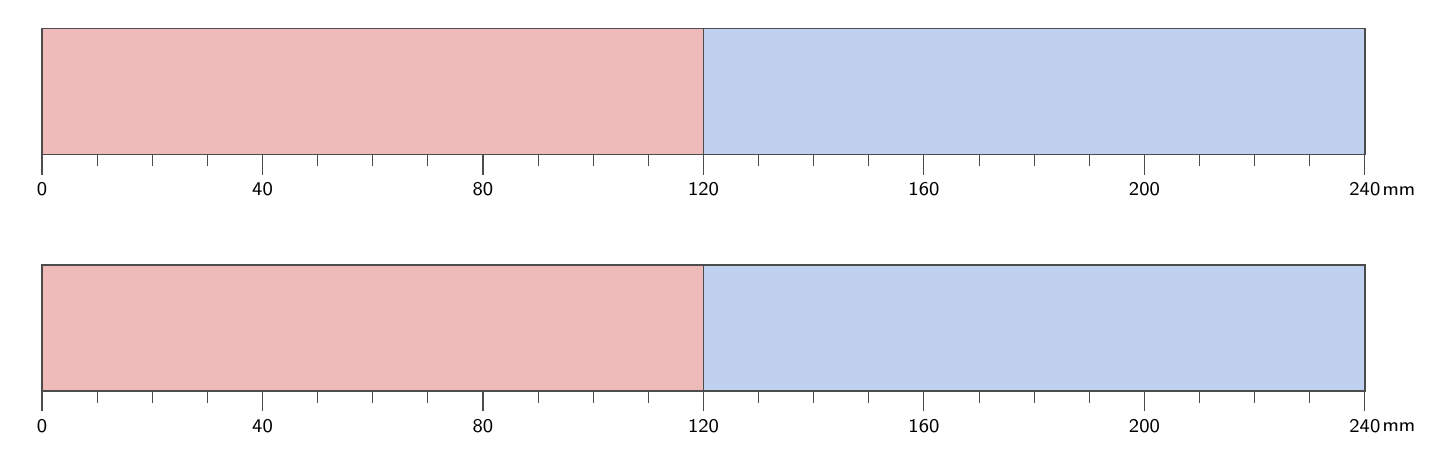
\begin{tikzpicture}[x=1mm,y=1mm]
\fill[stripred] (0,0) rectangle (84,16);
\fill[stripblue] (84,0) rectangle (168,16);
\draw[black!70, line width=0.6pt] (0,0) rectangle (168,16);
\draw[black!70, line width=0.6pt] (84,0) -- (84,16);
\draw[black!70, line width=0.4pt] (0,0) -- (0,-2.6);
\node[font=\scriptsize, below] at (0,-2.4) {0};
\draw[black!70, line width=0.4pt] (7,0) -- (7,-1.5);
\draw[black!70, line width=0.4pt] (14,0) -- (14,-1.5);
\draw[black!70, line width=0.4pt] (21,0) -- (21,-1.5);
\draw[black!70, line width=0.4pt] (28,0) -- (28,-2.6);
\node[font=\scriptsize, below] at (28,-2.4) {40};
\draw[black!70, line width=0.4pt] (35,0) -- (35,-1.5);
\draw[black!70, line width=0.4pt] (42,0) -- (42,-1.5);
\draw[black!70, line width=0.4pt] (49,0) -- (49,-1.5);
\draw[black!70, line width=0.4pt] (56,0) -- (56,-2.6);
\node[font=\scriptsize, below] at (56,-2.4) {80};
\draw[black!70, line width=0.4pt] (63,0) -- (63,-1.5);
\draw[black!70, line width=0.4pt] (70,0) -- (70,-1.5);
\draw[black!70, line width=0.4pt] (77,0) -- (77,-1.5);
\draw[black!70, line width=0.4pt] (84,0) -- (84,-2.6);
\node[font=\scriptsize, below] at (84,-2.4) {120};
\draw[black!70, line width=0.4pt] (91,0) -- (91,-1.5);
\draw[black!70, line width=0.4pt] (98,0) -- (98,-1.5);
\draw[black!70, line width=0.4pt] (105,0) -- (105,-1.5);
\draw[black!70, line width=0.4pt] (112,0) -- (112,-2.6);
\node[font=\scriptsize, below] at (112,-2.4) {160};
\draw[black!70, line width=0.4pt] (119,0) -- (119,-1.5);
\draw[black!70, line width=0.4pt] (126,0) -- (126,-1.5);
\draw[black!70, line width=0.4pt] (133,0) -- (133,-1.5);
\draw[black!70, line width=0.4pt] (140,0) -- (140,-2.6);
\node[font=\scriptsize, below] at (140,-2.4) {200};
\draw[black!70, line width=0.4pt] (147,0) -- (147,-1.5);
\draw[black!70, line width=0.4pt] (154,0) -- (154,-1.5);
\draw[black!70, line width=0.4pt] (161,0) -- (161,-1.5);
\draw[black!70, line width=0.4pt] (168,0) -- (168,-2.6);
\node[font=\scriptsize, below] at (168,-2.4) {240};
\node[font=\scriptsize, right] at (169,-4.6) {mm};
\fill[stripred] (0,-30) rectangle (84,-14);
\fill[stripblue] (84,-30) rectangle (168,-14);
\draw[black!70, line width=0.6pt] (0,-30) rectangle (168,-14);
\draw[black!70, line width=0.6pt] (84,-30) -- (84,-14);
\draw[black!70, line width=0.4pt] (0,-30) -- (0,-32.6);
\node[font=\scriptsize, below] at (0,-32.4) {0};
\draw[black!70, line width=0.4pt] (7,-30) -- (7,-31.5);
\draw[black!70, line width=0.4pt] (14,-30) -- (14,-31.5);
\draw[black!70, line width=0.4pt] (21,-30) -- (21,-31.5);
\draw[black!70, line width=0.4pt] (28,-30) -- (28,-32.6);
\node[font=\scriptsize, below] at (28,-32.4) {40};
\draw[black!70, line width=0.4pt] (35,-30) -- (35,-31.5);
\draw[black!70, line width=0.4pt] (42,-30) -- (42,-31.5);
\draw[black!70, line width=0.4pt] (49,-30) -- (49,-31.5);
\draw[black!70, line width=0.4pt] (56,-30) -- (56,-32.6);
\node[font=\scriptsize, below] at (56,-32.4) {80};
\draw[black!70, line width=0.4pt] (63,-30) -- (63,-31.5);
\draw[black!70, line width=0.4pt] (70,-30) -- (70,-31.5);
\draw[black!70, line width=0.4pt] (77,-30) -- (77,-31.5);
\draw[black!70, line width=0.4pt] (84,-30) -- (84,-32.6);
\node[font=\scriptsize, below] at (84,-32.4) {120};
\draw[black!70, line width=0.4pt] (91,-30) -- (91,-31.5);
\draw[black!70, line width=0.4pt] (98,-30) -- (98,-31.5);
\draw[black!70, line width=0.4pt] (105,-30) -- (105,-31.5);
\draw[black!70, line width=0.4pt] (112,-30) -- (112,-32.6);
\node[font=\scriptsize, below] at (112,-32.4) {160};
\draw[black!70, line width=0.4pt] (119,-30) -- (119,-31.5);
\draw[black!70, line width=0.4pt] (126,-30) -- (126,-31.5);
\draw[black!70, line width=0.4pt] (133,-30) -- (133,-31.5);
\draw[black!70, line width=0.4pt] (140,-30) -- (140,-32.6);
\node[font=\scriptsize, below] at (140,-32.4) {200};
\draw[black!70, line width=0.4pt] (147,-30) -- (147,-31.5);
\draw[black!70, line width=0.4pt] (154,-30) -- (154,-31.5);
\draw[black!70, line width=0.4pt] (161,-30) -- (161,-31.5);
\draw[black!70, line width=0.4pt] (168,-30) -- (168,-32.6);
\node[font=\scriptsize, below] at (168,-32.4) {240};
\node[font=\scriptsize, right] at (169,-34.6) {mm};
\end{tikzpicture}
\end{center}
\newpage
\prob{4}Three people use the three-person cards A, B and C, which give these values to the grey panels X, Y and Z.
\begin{center}
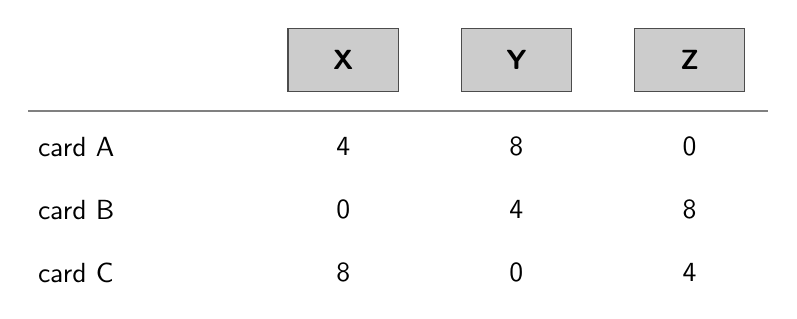
\begin{tikzpicture}[x=1mm,y=1mm]
\draw[black!70, fill=panelgrey, line width=0.5pt] (33,-8) rectangle (47,0);
\node[font=\bfseries] at (40,-4) {X};
\draw[black!70, fill=panelgrey, line width=0.5pt] (55,-8) rectangle (69,0);
\node[font=\bfseries] at (62,-4) {Y};
\draw[black!70, fill=panelgrey, line width=0.5pt] (77,-8) rectangle (91,0);
\node[font=\bfseries] at (84,-4) {Z};
\node[anchor=west] at (0,-15) {card A};
\node at (40,-15) {4};
\node at (62,-15) {8};
\node at (84,-15) {0};
\node[anchor=west] at (0,-23) {card B};
\node at (40,-23) {0};
\node at (62,-23) {4};
\node at (84,-23) {8};
\node[anchor=west] at (0,-31) {card C};
\node at (40,-31) {8};
\node at (62,-31) {0};
\node at (84,-31) {4};
\draw[black!50, line width=0.4pt] (0,-10.5) -- (94,-10.5);
\end{tikzpicture}
\end{center}
Each number is the value of a whole 50\,mm panel. A panel may be cut straight across, and value follows length within a panel:
\begin{center}
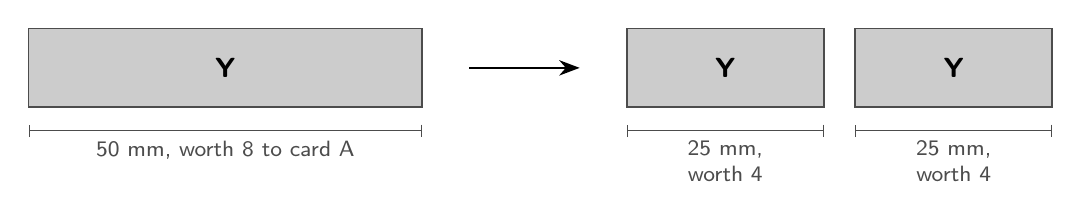
\begin{tikzpicture}[x=1mm,y=1mm]
\draw[black!70, fill=panelgrey, line width=0.6pt] (0,0) rectangle (50,10);
\node[font=\bfseries] at (25,5) {Y};
\draw[|-|, black!70, line width=0.4pt] (0,-3) -- node[below, font=\footnotesize] {50 mm, worth 8 to card A} (50,-3);
\draw[-{Stealth[length=2.6mm]}, line width=0.9pt] (56,5) -- (70,5);
\draw[black!70, fill=panelgrey, line width=0.6pt] (76,0) rectangle (101,10);
\node[font=\bfseries] at (88.5,5) {Y};
\draw[|-|, black!70, line width=0.4pt] (76,-3) -- node[below, font=\footnotesize, align=center] {25 mm,\\ worth 4} (101,-3);
\draw[black!70, fill=panelgrey, line width=0.6pt] (105,0) rectangle (130,10);
\node[font=\bfseries] at (117.5,5) {Y};
\draw[|-|, black!70, line width=0.4pt] (105,-3) -- node[below, font=\footnotesize, align=center] {25 mm,\\ worth 4} (130,-3);
\end{tikzpicture}
\end{center}
Lay the panels in the row X~Y~Z. Share the row between two trays so that each of the three people finds the two trays worth the same. Use as few cuts as you can, and explain why fewer cuts cannot work.
\vspace{4mm}
\begin{center}
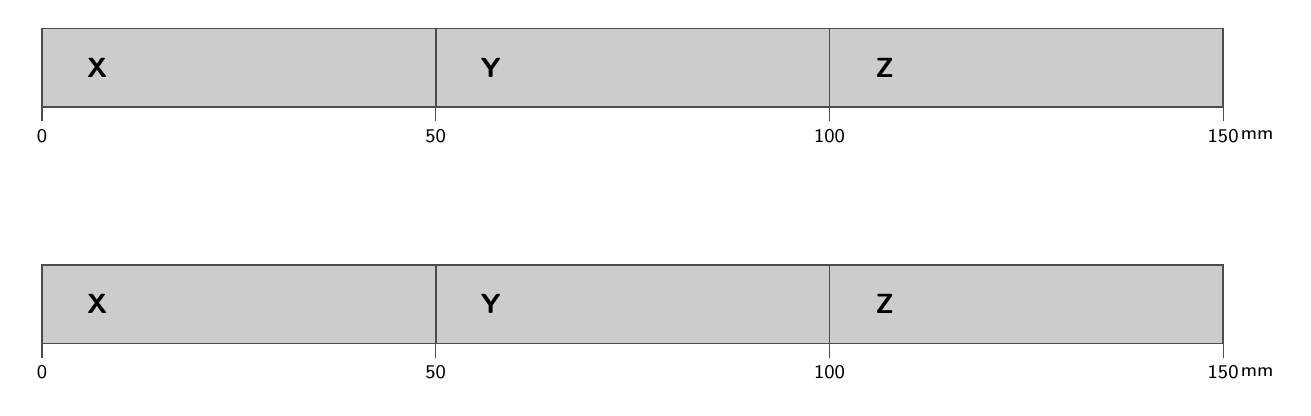
\begin{tikzpicture}[x=1mm,y=1mm]
\draw[black!70, fill=panelgrey, line width=0.6pt] (0,0) rectangle (50,10);
\node[font=\bfseries] at (7,5) {X};
\draw[black!70, fill=panelgrey, line width=0.6pt] (50,0) rectangle (100,10);
\node[font=\bfseries] at (57,5) {Y};
\draw[black!70, fill=panelgrey, line width=0.6pt] (100,0) rectangle (150,10);
\node[font=\bfseries] at (107,5) {Z};
\draw[black!70, line width=0.4pt] (0,0) -- (0,-1.8);
\node[font=\scriptsize, below] at (0,-1.6) {0};
\draw[black!70, line width=0.4pt] (50,0) -- (50,-1.8);
\node[font=\scriptsize, below] at (50,-1.6) {50};
\draw[black!70, line width=0.4pt] (100,0) -- (100,-1.8);
\node[font=\scriptsize, below] at (100,-1.6) {100};
\draw[black!70, line width=0.4pt] (150,0) -- (150,-1.8);
\node[font=\scriptsize, below] at (150,-1.6) {150};
\node[font=\scriptsize, right] at (151,-3.6) {mm};
\draw[black!70, fill=panelgrey, line width=0.6pt] (0,-30) rectangle (50,-20);
\node[font=\bfseries] at (7,-25) {X};
\draw[black!70, fill=panelgrey, line width=0.6pt] (50,-30) rectangle (100,-20);
\node[font=\bfseries] at (57,-25) {Y};
\draw[black!70, fill=panelgrey, line width=0.6pt] (100,-30) rectangle (150,-20);
\node[font=\bfseries] at (107,-25) {Z};
\draw[black!70, line width=0.4pt] (0,-30) -- (0,-31.8);
\node[font=\scriptsize, below] at (0,-31.6) {0};
\draw[black!70, line width=0.4pt] (50,-30) -- (50,-31.8);
\node[font=\scriptsize, below] at (50,-31.6) {50};
\draw[black!70, line width=0.4pt] (100,-30) -- (100,-31.8);
\node[font=\scriptsize, below] at (100,-31.6) {100};
\draw[black!70, line width=0.4pt] (150,-30) -- (150,-31.8);
\node[font=\scriptsize, below] at (150,-31.6) {150};
\node[font=\scriptsize, right] at (151,-33.6) {mm};
\end{tikzpicture}
\end{center}
\newpage
\prob{5}The same three people share the row with a marking game. Each person marks where the piece from the left end first becomes worth 4 by their own card, a third of their total. Whoever marked leftmost takes that piece. The other two mark again from the new left end, aiming at 4 again, and whoever marked leftmost takes that piece. The last person takes the rest. If two marks are at the same place, either of those people may take the piece.
\begin{center}
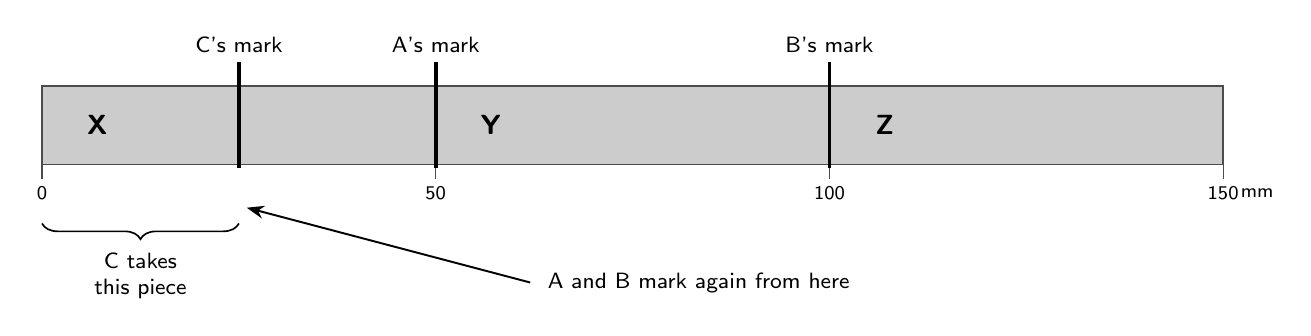
\begin{tikzpicture}[x=1mm,y=1mm]
\draw[black!70, fill=panelgrey, line width=0.6pt] (0,0) rectangle (50,10);
\node[font=\bfseries] at (7,5) {X};
\draw[black!70, fill=panelgrey, line width=0.6pt] (50,0) rectangle (100,10);
\node[font=\bfseries] at (57,5) {Y};
\draw[black!70, fill=panelgrey, line width=0.6pt] (100,0) rectangle (150,10);
\node[font=\bfseries] at (107,5) {Z};
\draw[black!70, line width=0.4pt] (0,0) -- (0,-1.8);
\node[font=\scriptsize, below] at (0,-1.6) {0};
\draw[black!70, line width=0.4pt] (50,0) -- (50,-1.8);
\node[font=\scriptsize, below] at (50,-1.6) {50};
\draw[black!70, line width=0.4pt] (100,0) -- (100,-1.8);
\node[font=\scriptsize, below] at (100,-1.6) {100};
\draw[black!70, line width=0.4pt] (150,0) -- (150,-1.8);
\node[font=\scriptsize, below] at (150,-1.6) {150};
\node[font=\scriptsize, right] at (151,-3.6) {mm};
\draw[black, line width=1.3pt] (25,-0.5) -- (25,13);
\node[font=\footnotesize, above] at (25,13) {C's mark};
\draw[black, line width=1.3pt] (50,-0.5) -- (50,13);
\node[font=\footnotesize, above] at (50,13) {A's mark};
\draw[black, line width=1.3pt] (100,-0.5) -- (100,13);
\node[font=\footnotesize, above] at (100,13) {B's mark};
\draw[decorate, decoration={brace, amplitude=2mm, mirror}, line width=0.6pt] (0,-7.5) -- (25,-7.5);
\node[font=\footnotesize, align=center, below] at (12.5,-10) {C takes\\this piece};
\draw[-{Stealth[length=2.2mm]}, line width=0.7pt] (62,-15) -- (26,-5.5);
\node[font=\footnotesize, anchor=west] at (63,-15) {A and B mark again from here};
\end{tikzpicture}
\end{center}
Finish this game, and play the game with the panels in each of the other five orders. Does anyone get less than 4 by their own card? Would anyone rather have someone else's piece?
\vspace{2mm}
\begin{center}
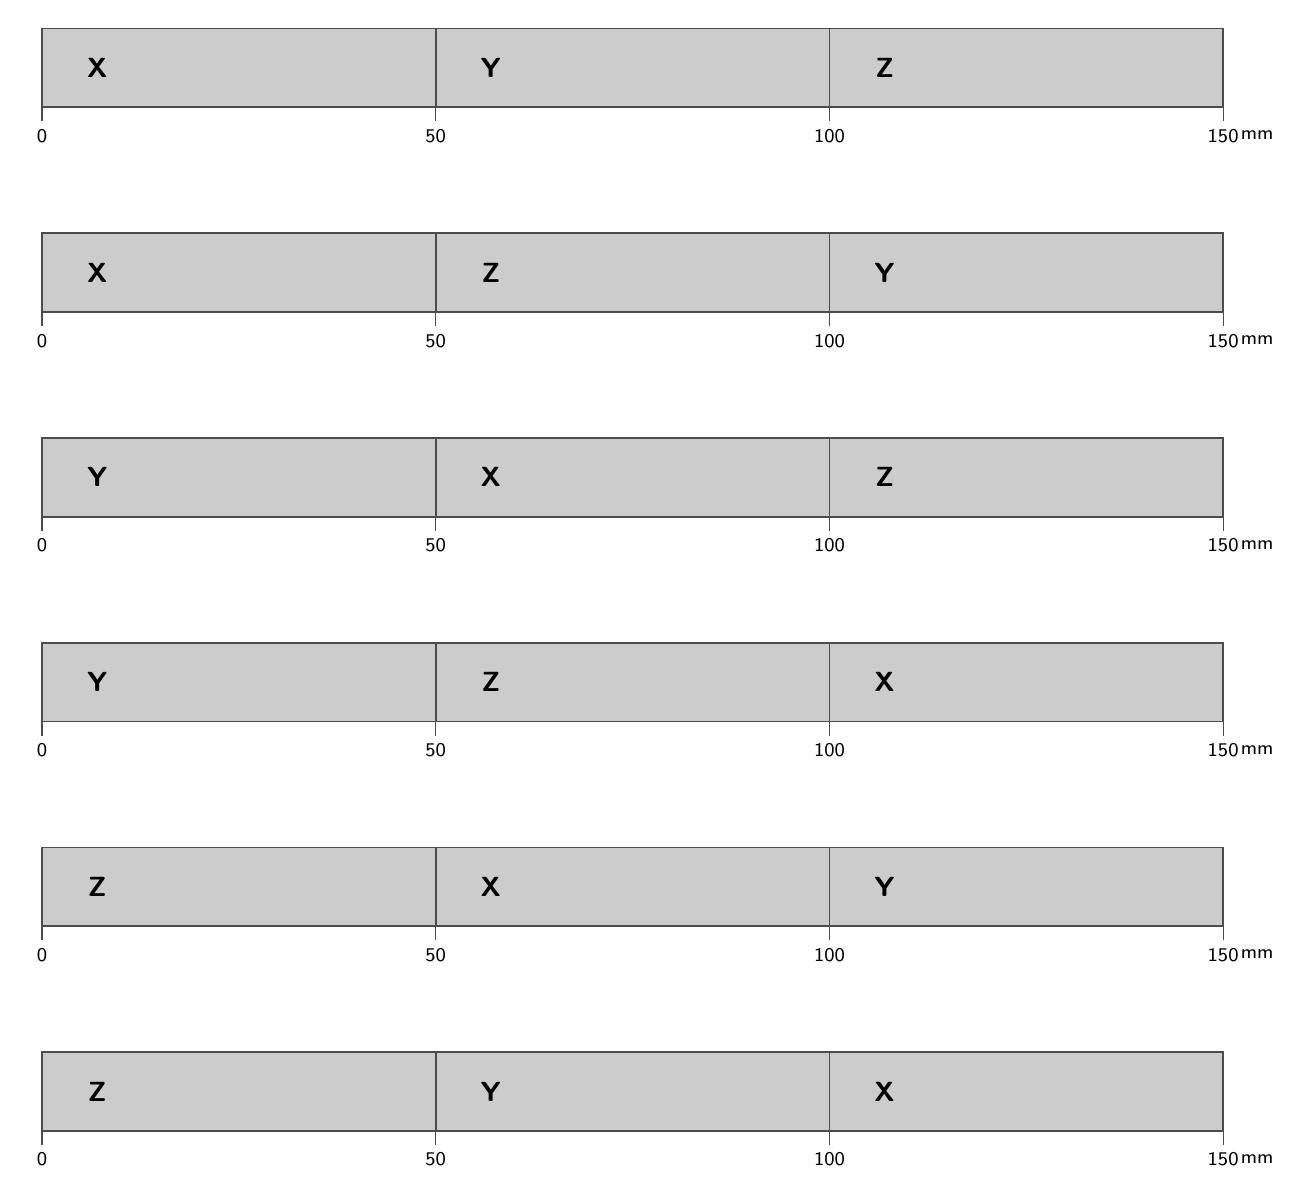
\begin{tikzpicture}[x=1mm,y=1mm]
\draw[black!70, fill=panelgrey, line width=0.6pt] (0,0) rectangle (50,10);
\node[font=\bfseries] at (7,5) {X};
\draw[black!70, fill=panelgrey, line width=0.6pt] (50,0) rectangle (100,10);
\node[font=\bfseries] at (57,5) {Y};
\draw[black!70, fill=panelgrey, line width=0.6pt] (100,0) rectangle (150,10);
\node[font=\bfseries] at (107,5) {Z};
\draw[black!70, line width=0.4pt] (0,0) -- (0,-1.8);
\node[font=\scriptsize, below] at (0,-1.6) {0};
\draw[black!70, line width=0.4pt] (50,0) -- (50,-1.8);
\node[font=\scriptsize, below] at (50,-1.6) {50};
\draw[black!70, line width=0.4pt] (100,0) -- (100,-1.8);
\node[font=\scriptsize, below] at (100,-1.6) {100};
\draw[black!70, line width=0.4pt] (150,0) -- (150,-1.8);
\node[font=\scriptsize, below] at (150,-1.6) {150};
\node[font=\scriptsize, right] at (151,-3.6) {mm};
\draw[black!70, fill=panelgrey, line width=0.6pt] (0,-26) rectangle (50,-16);
\node[font=\bfseries] at (7,-21) {X};
\draw[black!70, fill=panelgrey, line width=0.6pt] (50,-26) rectangle (100,-16);
\node[font=\bfseries] at (57,-21) {Z};
\draw[black!70, fill=panelgrey, line width=0.6pt] (100,-26) rectangle (150,-16);
\node[font=\bfseries] at (107,-21) {Y};
\draw[black!70, line width=0.4pt] (0,-26) -- (0,-27.8);
\node[font=\scriptsize, below] at (0,-27.6) {0};
\draw[black!70, line width=0.4pt] (50,-26) -- (50,-27.8);
\node[font=\scriptsize, below] at (50,-27.6) {50};
\draw[black!70, line width=0.4pt] (100,-26) -- (100,-27.8);
\node[font=\scriptsize, below] at (100,-27.6) {100};
\draw[black!70, line width=0.4pt] (150,-26) -- (150,-27.8);
\node[font=\scriptsize, below] at (150,-27.6) {150};
\node[font=\scriptsize, right] at (151,-29.6) {mm};
\draw[black!70, fill=panelgrey, line width=0.6pt] (0,-52) rectangle (50,-42);
\node[font=\bfseries] at (7,-47) {Y};
\draw[black!70, fill=panelgrey, line width=0.6pt] (50,-52) rectangle (100,-42);
\node[font=\bfseries] at (57,-47) {X};
\draw[black!70, fill=panelgrey, line width=0.6pt] (100,-52) rectangle (150,-42);
\node[font=\bfseries] at (107,-47) {Z};
\draw[black!70, line width=0.4pt] (0,-52) -- (0,-53.8);
\node[font=\scriptsize, below] at (0,-53.6) {0};
\draw[black!70, line width=0.4pt] (50,-52) -- (50,-53.8);
\node[font=\scriptsize, below] at (50,-53.6) {50};
\draw[black!70, line width=0.4pt] (100,-52) -- (100,-53.8);
\node[font=\scriptsize, below] at (100,-53.6) {100};
\draw[black!70, line width=0.4pt] (150,-52) -- (150,-53.8);
\node[font=\scriptsize, below] at (150,-53.6) {150};
\node[font=\scriptsize, right] at (151,-55.6) {mm};
\draw[black!70, fill=panelgrey, line width=0.6pt] (0,-78) rectangle (50,-68);
\node[font=\bfseries] at (7,-73) {Y};
\draw[black!70, fill=panelgrey, line width=0.6pt] (50,-78) rectangle (100,-68);
\node[font=\bfseries] at (57,-73) {Z};
\draw[black!70, fill=panelgrey, line width=0.6pt] (100,-78) rectangle (150,-68);
\node[font=\bfseries] at (107,-73) {X};
\draw[black!70, line width=0.4pt] (0,-78) -- (0,-79.8);
\node[font=\scriptsize, below] at (0,-79.6) {0};
\draw[black!70, line width=0.4pt] (50,-78) -- (50,-79.8);
\node[font=\scriptsize, below] at (50,-79.6) {50};
\draw[black!70, line width=0.4pt] (100,-78) -- (100,-79.8);
\node[font=\scriptsize, below] at (100,-79.6) {100};
\draw[black!70, line width=0.4pt] (150,-78) -- (150,-79.8);
\node[font=\scriptsize, below] at (150,-79.6) {150};
\node[font=\scriptsize, right] at (151,-81.6) {mm};
\draw[black!70, fill=panelgrey, line width=0.6pt] (0,-104) rectangle (50,-94);
\node[font=\bfseries] at (7,-99) {Z};
\draw[black!70, fill=panelgrey, line width=0.6pt] (50,-104) rectangle (100,-94);
\node[font=\bfseries] at (57,-99) {X};
\draw[black!70, fill=panelgrey, line width=0.6pt] (100,-104) rectangle (150,-94);
\node[font=\bfseries] at (107,-99) {Y};
\draw[black!70, line width=0.4pt] (0,-104) -- (0,-105.8);
\node[font=\scriptsize, below] at (0,-105.6) {0};
\draw[black!70, line width=0.4pt] (50,-104) -- (50,-105.8);
\node[font=\scriptsize, below] at (50,-105.6) {50};
\draw[black!70, line width=0.4pt] (100,-104) -- (100,-105.8);
\node[font=\scriptsize, below] at (100,-105.6) {100};
\draw[black!70, line width=0.4pt] (150,-104) -- (150,-105.8);
\node[font=\scriptsize, below] at (150,-105.6) {150};
\node[font=\scriptsize, right] at (151,-107.6) {mm};
\draw[black!70, fill=panelgrey, line width=0.6pt] (0,-130) rectangle (50,-120);
\node[font=\bfseries] at (7,-125) {Z};
\draw[black!70, fill=panelgrey, line width=0.6pt] (50,-130) rectangle (100,-120);
\node[font=\bfseries] at (57,-125) {Y};
\draw[black!70, fill=panelgrey, line width=0.6pt] (100,-130) rectangle (150,-120);
\node[font=\bfseries] at (107,-125) {X};
\draw[black!70, line width=0.4pt] (0,-130) -- (0,-131.8);
\node[font=\scriptsize, below] at (0,-131.6) {0};
\draw[black!70, line width=0.4pt] (50,-130) -- (50,-131.8);
\node[font=\scriptsize, below] at (50,-131.6) {50};
\draw[black!70, line width=0.4pt] (100,-130) -- (100,-131.8);
\node[font=\scriptsize, below] at (100,-131.6) {100};
\draw[black!70, line width=0.4pt] (150,-130) -- (150,-131.8);
\node[font=\scriptsize, below] at (150,-131.6) {150};
\node[font=\scriptsize, right] at (151,-133.6) {mm};
\end{tikzpicture}
\end{center}
\newpage
\prob{6}Explain why the marking game gives each person at least a third of their own total, whatever the order of the panels and whatever values the cards give. Giving A the whole Y, B the whole Z and C the whole X gives each of them 8 by their own card. Can the game ever do that well for all three?
\vspace{80mm}
\prob{7}Lay the goods cards touching in this row, using the paper R3. Here a card may be cut straight across, and its value is spread evenly from its left edge to its right edge.
\begin{center}
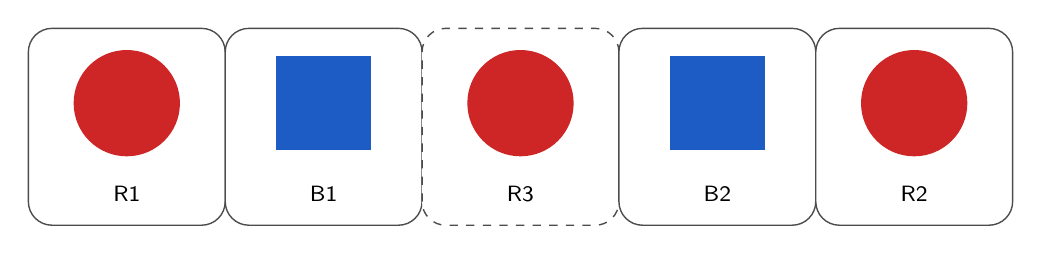
\begin{tikzpicture}[x=1mm,y=1mm]
\draw[cardedge, fill=white, rounded corners=3mm] (0,0) rectangle (25,25);
\fill[cardred] (12.5,15.5) circle (6.75mm);
\node[font=\footnotesize] at (12.5,4) {R1};
\draw[cardedge, fill=white, rounded corners=3mm] (25,0) rectangle (50,25);
\fill[cardblue] (31.5,9.5) rectangle (43.5,21.5);
\node[font=\footnotesize] at (37.5,4) {B1};
\draw[draw=black!70, line width=0.5pt, dashed, fill=white, rounded corners=3mm] (50,0) rectangle (75,25);
\fill[cardred] (62.5,15.5) circle (6.75mm);
\node[font=\footnotesize] at (62.5,4) {R3};
\draw[cardedge, fill=white, rounded corners=3mm] (75,0) rectangle (100,25);
\fill[cardblue] (81.5,9.5) rectangle (93.5,21.5);
\node[font=\footnotesize] at (87.5,4) {B2};
\draw[cardedge, fill=white, rounded corners=3mm] (100,0) rectangle (125,25);
\fill[cardred] (112.5,15.5) circle (6.75mm);
\node[font=\footnotesize] at (112.5,4) {R2};
\end{tikzpicture}
\end{center}
Two people both use the two-person card A. Where should one cut go so that each of them gets exactly half of the total by card A? Can you arrange the five cards so that the cut falls between two cards, or inside a blue card?
\newpage
\prob{8}Explain why the marking game for three people, on any row of whole goods cards, never cuts more than two cards. Three people all value every red card at 1 and every blue card at 0, as card U does. They share two paper red cards lying side by side. Can each of them get at least a third of the total while only one card is cut?

\end{document}
